\documentclass{standalone}

\usepackage{tikz}

\begin{document}
  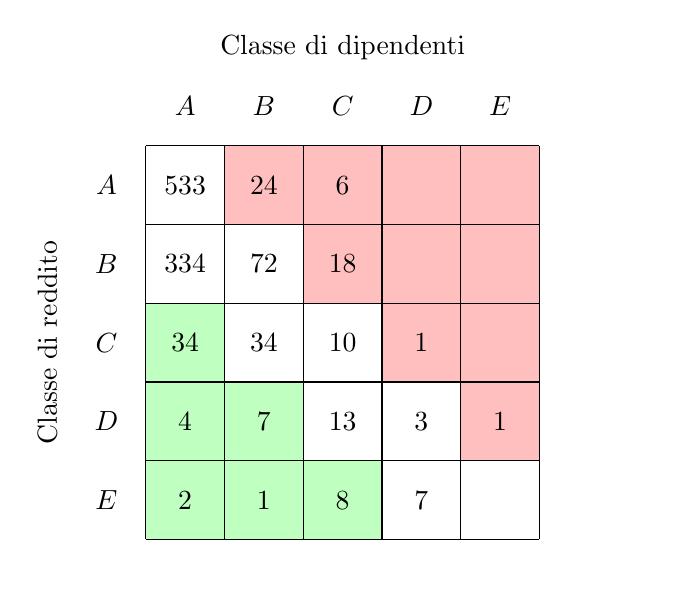
\begin{tikzpicture}
    \path[use as bounding box] (-0.5,0.5) rectangle (7.5,7.5);

    \fill [fill=green!25] (1,1) -- (4,1) -- (4,2) -- (3,2) -- (3,3) -- (2,3) -- (2,4) -- (1,4) -- cycle;
    \fill [fill=red!25] (6,6) -- (6,2) -- (5,2) -- (5,3) -- (4,3) -- (4,4) -- (3,4) -- (3,5) -- (2,5) -- (2,6) -- cycle;

    \node (revenue-label) at (3.5,7.25) [] {Classe di dipendenti};
    \node (employee-label) at (-0.25,3.5) [rotate=90] {Classe di reddito};

    \node (A-employee) at (1.5,6.5) [] {\(A\)};
    \node (B-employee) at (2.5,6.5) [] {\(B\)};
    \node (C-employee) at (3.5,6.5) [] {\(C\)};
    \node (D-employee) at (4.5,6.5) [] {\(D\)};
    \node (E-employee) at (5.5,6.5) [] {\(E\)};

    \node (A-revenue) at (0.5,5.5) [] {\(A\)};
    \node (B-revenue) at (0.5,4.5) [] {\(B\)};
    \node (C-revenue) at (0.5,3.5) [] {\(C\)};
    \node (D-revenue) at (0.5,2.5) [] {\(D\)};
    \node (E-revenue) at (0.5,1.5) [] {\(E\)};

    \node (AA-data) at (1.5,5.5) [] {\(533\)};
    \node (AB-data) at (2.5,5.5) [] {\(24\)};
    \node (AC-data) at (3.5,5.5) [] {\(6\)};
    \node (AD-data) at (4.5,5.5) [] {};
    \node (AE-data) at (5.5,5.5) [] {};

    \node (BA-data) at (1.5,4.5) [] {\(334\)};
    \node (BB-data) at (2.5,4.5) [] {\(72\)};
    \node (BC-data) at (3.5,4.5) [] {\(18\)};
    \node (BD-data) at (4.5,4.5) [] {};
    \node (BE-data) at (5.5,4.5) [] {};

    \node (CA-data) at (1.5,3.5) [] {\(34\)};
    \node (CB-data) at (2.5,3.5) [] {\(34\)};
    \node (CC-data) at (3.5,3.5) [] {\(10\)};
    \node (CD-data) at (4.5,3.5) [] {\(1\)};
    \node (CE-data) at (5.5,3.5) [] {};

    \node (DA-data) at (1.5,2.5) [] {\(4\)};
    \node (DB-data) at (2.5,2.5) [] {\(7\)};
    \node (DC-data) at (3.5,2.5) [] {\(13\)};
    \node (DD-data) at (4.5,2.5) [] {\(3\)};
    \node (DE-data) at (5.5,2.5) [] {\(1\)};

    \node (EA-data) at (1.5,1.5) [] {\(2\)};
    \node (EB-data) at (2.5,1.5) [] {\(1\)};
    \node (EC-data) at (3.5,1.5) [] {\(8\)};
    \node (ED-data) at (4.5,1.5) [] {\(7\)};
    \node (EE-data) at (5.5,1.5) [] {};

    \draw (1,1) -- (6,1);
    \draw (1,2) -- (6,2);
    \draw (1,3) -- (6,3);
    \draw (1,4) -- (6,4);
    \draw (1,5) -- (6,5);
    \draw (1,6) -- (6,6);

    \draw (1,1) -- (1,6);
    \draw (2,1) -- (2,6);
    \draw (3,1) -- (3,6);
    \draw (4,1) -- (4,6);
    \draw (5,1) -- (5,6);
    \draw (6,1) -- (6,6);
  \end{tikzpicture}
\end{document}
